\documentclass[12pt,a4paper]{article}

\usepackage[T1]{fontenc}
\usepackage[utf8]{inputenc}
\usepackage{lmodern}
\usepackage{microtype}
\usepackage[a4paper,margin=2.54cm]{geometry}
\usepackage{amsmath,amssymb}
\usepackage{array}
\usepackage{xcolor}
\usepackage{booktabs}
\usepackage{setspace}
\usepackage[hidelinks]{hyperref}
\usepackage{tikz}
\usetikzlibrary{positioning,arrows.meta}

\setlength{\parindent}{1.5em}
\setlength{\parskip}{0pt}
\setlength{\emergencystretch}{2em}
\newcolumntype{P}[1]{>{\raggedright\arraybackslash}p{#1}}

\begin{document}

\begin{center}
    {\Large\bfseries
    Physics-Guided Allocation of Conductive Particles in Granular Beds:\par
    A Hybrid DEM, Thermal-Network and Graph-Learning Framework\par}
    \vspace{1.25em}
    {\normalsize Ali Khalifa and Heba Alzaben\par}
    \vspace{0.6em}
    {\small Technical University of Munich, Freising, Germany;\par
    Al Hussein Technical University, Amman, Jordan\par}
\end{center}

\vspace{1.25em}
\setstretch{1.5}

\begin{abstract}
The effective thermal conductivity of a granular bed is governed not only by
porosity, particle-size distribution and constituent conductivities, but also
by the topology of the particle contact network. In a binary bed containing a
limited fraction of highly conductive particles, the same material fraction
can therefore produce different heat-transfer performance depending on where
those particles are placed. Existing thermal discrete-element and resistance-
network models mainly evaluate the forward relation from an already specified
packing and material distribution to heat transfer. Conversely, graph-learning
and inverse-design studies have generally focused on continuous or architected
materials rather than discrete material allocation on mechanically realizable
granular contact networks. This study proposes a hybrid framework in which the
discrete-element method (DEM) generates physically admissible packings, a
steady thermal resistor network provides exact and inexpensive physics labels,
and graph-based optimization identifies which particles should receive a
high-conductivity material under a fixed material budget. The thermal network
contains both solid-contact conduction and conduction through a stagnant
interstitial fluid; no imposed fluid motion or convective transport is assumed.
Random allocation,
degree and centrality rankings, continuous-relaxation methods and greedy
physics-based selection provide mandatory baselines. A graph neural network
(GNN) is introduced only if it can learn a transferable placement policy that
generalizes to unseen DEM packings or larger systems. The central hypothesis is
that conductivity enhancement depends on the formation of boundary-spanning,
low-resistance pathways and cannot be determined reliably from porosity,
particle-size distribution or isolated node scores alone. An initial pilot uses
ten independent 500-particle packings with identical number-based particle-size
distribution and nominal porosity. The intended outcome is a reproducible
physics-guided design rule for allocating a limited conductive phase in
granular thermal-storage or heat-transfer media, together with quantitative
evidence of when learned graph policies add value beyond conventional network
heuristics.
\end{abstract}

\noindent\textbf{Keywords:} granular beds; discrete-element method; thermal
resistor network; effective thermal conductivity; material allocation; graph
neural network; inverse design; hybrid modelling

\section{Motivation, research gap and hypothesis}

Heat conduction through granular media is controlled by particle properties,
contact areas, packing density, interstitial phases and the organization of the
contact network. Classical studies and more recent thermal DEM formulations
have established physically meaningful forward models for conduction through
particle assemblies \cite{Batchelor1977,Vargas2001,Kiani2019}. These models can
resolve packing heterogeneity more directly than correlations based only on
bulk porosity or coordination number. They do not, however, automatically
answer an inverse design question: given a mechanically fixed packing and a
limited quantity of an expensive conductive material, which particles should
be made conductive to maximize heat transfer between two boundaries?

This distinction is important. If the fraction of conductive particles is
fixed, random mixing may waste material in isolated clusters, transverse
branches or redundant parts of an already conductive pathway. Selecting the
highest-degree particles is also not necessarily optimal, because a locally
well-connected node can be poorly positioned relative to the hot and cold
boundaries. The useful arrangement must account simultaneously for local
connectivity, particle size, contact conductance, direction relative to the
temperature gradient, and the global formation of competing or complementary
paths through the bed.

Graph-based inverse design has been demonstrated for architected lattice
materials, including differentiable message-passing approaches that modify
local graph attributes to achieve target properties \cite{Dold2023}. The
proposed study is different in both physical system and design variable. The
graph is not an arbitrary lattice to be generated or geometrically deformed;
it is a contact network produced by DEM at prescribed porosity and particle-
size distribution. Its geometry remains fixed, and the inverse problem is a
binary, fixed-budget assignment of particle material. The scientific question
is therefore whether a small conductive phase can be allocated more effectively
by exploiting the actual topology of a realizable granular packing.

The central hypothesis is:
\begin{quote}
For granular beds with identical porosity, particle-size distribution and
conductive-particle fraction, effective conductivity depends strongly on the
global arrangement of the conductive phase. Boundary-aware, cooperative
selection of particles can create low-resistance spanning pathways that cannot
be identified reliably by random allocation or isolated node-centrality scores.
\end{quote}

This hypothesis is falsifiable. If optimized assignments do not consistently
outperform random and simple heuristic allocations across unseen packings, the
placement problem is not practically important in the investigated regime. If
a deterministic physics-based algorithm performs as well as a GNN, the graph
learning component is unnecessary and should not be presented as the main
contribution.

\section{Hybrid modelling concept and novelty}

The framework separates three roles. DEM generates mechanically realizable
particle positions, sizes and contacts. A thermal-network solver evaluates any
material assignment by enforcing energy conservation. Optimization or graph
learning searches the discrete assignment space without replacing the physical
thermal model.

For a packing graph $\mathcal G=(\mathcal V,\mathcal E)$, let
$x_i\in\{0,1\}$ indicate whether particle $i$ is assigned the high-conductivity
material. The fixed material budget is
\begin{equation}
    \sum_{i\in\mathcal V}x_i=M,
    \label{eq:budget}
\end{equation}
where $M$ is the prescribed number of conductive particles. Particle
conductivity is then
\begin{equation}
    k_i=k_{\mathrm L}+
    x_i\left(k_{\mathrm H}-k_{\mathrm L}\right).
\end{equation}
For every internal particle, steady energy conservation requires
\begin{equation}
    \sum_{j\in\mathcal N_i}G_{ij}(T_j-T_i)=0,
    \label{eq:energy_balance}
\end{equation}
where $G_{ij}$ is the total solid-contact and stagnant-fluid conductance between
neighbouring particles $i$ and $j$. After applying hot and cold
boundary temperatures, the resulting heat rate $Q$ gives
\begin{equation}
    k_{\mathrm{eff}}=\frac{QH}{A\left(T_{\mathrm h}-T_{\mathrm c}\right)}.
    \label{eq:keff}
\end{equation}
The inverse problem is
\begin{equation}
    \mathbf x^{*}=\underset{\mathbf x\in\{0,1\}^{N}}
    {\operatorname{arg\,max}}\;
    k_{\mathrm{eff}}(\mathcal G,\mathbf x)
    \quad\text{subject to Eq.~\eqref{eq:budget}.}
    \label{eq:inverse}
\end{equation}

The main novelty is not the separate use of DEM, network conduction or a GNN.
It is the controlled inverse allocation of a fixed conductive-particle budget
directly on multiple physically realizable DEM contact networks, with the
thermal equations retained as the evaluator. The study will quantify which
topological mechanisms make an allocation effective, whether optimal patterns
transfer across stochastic packings, and whether graph learning offers a
reproducible advantage over transparent physics and network baselines. This is
more specific and defensible than claiming the first use of machine learning
for granular thermal conductivity.

Figure~\ref{fig:problem} illustrates the physical problem. The particle geometry
and contact topology are fixed after DEM generation. Only the binary material
labels are changed. Heat can pass through direct solid contacts and through the
stationary fluid occupying the void space. The latter contributes thermal
conduction without requiring fluid motion or CFD.

\begin{figure}[!htbp]
\centering
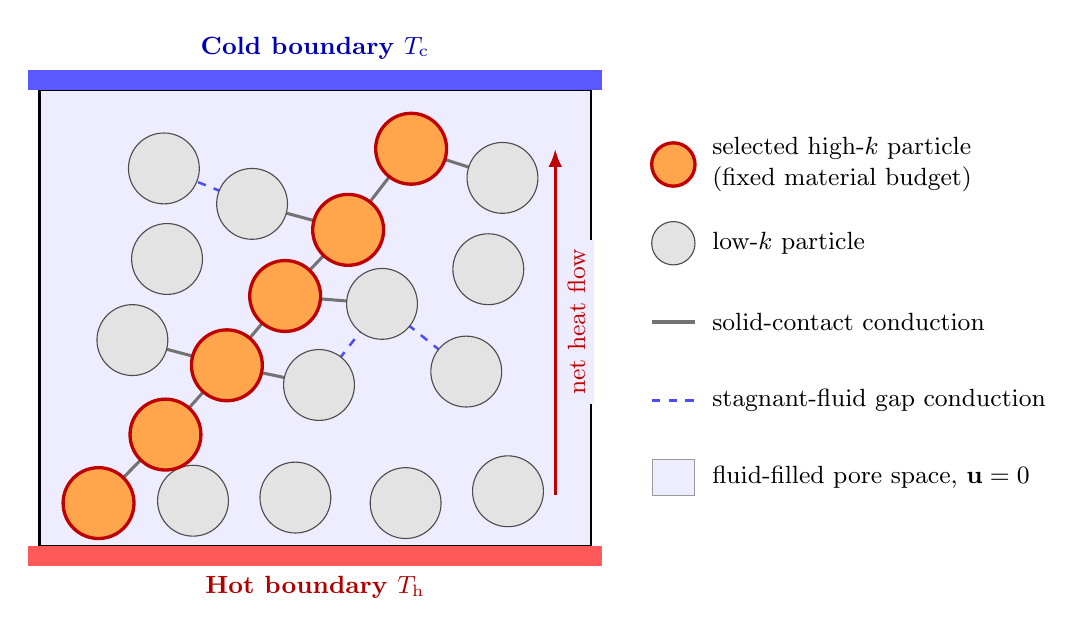
\begin{tikzpicture}[
particle/.style={circle,draw=black!70,fill=gray!22,minimum size=9mm,inner sep=0pt},
conductive/.style={circle,draw=red!75!black,very thick,fill=orange!70,minimum size=9mm,inner sep=0pt},
contact/.style={draw=black!55,line width=1.1pt},
gap/.style={draw=blue!70,dashed,line width=0.9pt},
heat/.style={-{Latex[length=2.3mm]},red!75!black,very thick},
labelbox/.style={align=left,font=\small}
]
\fill[blue!7] (0,0) rectangle (7,5.8);
\draw[thick] (0,0) rectangle (7,5.8);
\fill[red!65] (-0.15,-0.25) rectangle (7.15,0);
\fill[blue!65] (-0.15,5.8) rectangle (7.15,6.05);
\node[font=\small\bfseries,red!70!black] at (3.5,-0.52) {Hot boundary $T_{\mathrm h}$};
\node[font=\small\bfseries,blue!70!black] at (3.5,6.33) {Cold boundary $T_{\mathrm c}$};

\draw[contact] (0.75,0.55)--(1.60,1.42)--(2.38,2.30)--(3.12,3.18)--(3.92,4.02)--(4.72,5.05);
\draw[contact] (1.95,0.58)--(1.60,1.42);
\draw[contact] (2.38,2.30)--(1.18,2.62);
\draw[contact] (2.38,2.30)--(3.55,2.05);
\draw[contact] (3.12,3.18)--(4.35,3.08);
\draw[contact] (3.92,4.02)--(2.70,4.35);
\draw[contact] (4.72,5.05)--(5.88,4.68);
\draw[gap] (3.55,2.05)--(4.35,3.08);
\draw[gap] (4.35,3.08)--(5.42,2.22);
\draw[gap] (2.70,4.35)--(1.58,4.80);

\node[particle] at (1.95,0.58) {};
\node[particle] at (3.25,0.62) {};
\node[particle] at (4.65,0.55) {};
\node[particle] at (5.95,0.70) {};
\node[particle] at (1.18,2.62) {};
\node[particle] at (3.55,2.05) {};
\node[particle] at (5.42,2.22) {};
\node[particle] at (1.62,3.65) {};
\node[particle] at (4.35,3.08) {};
\node[particle] at (5.70,3.52) {};
\node[particle] at (2.70,4.35) {};
\node[particle] at (1.58,4.80) {};
\node[particle] at (5.88,4.68) {};

\node[conductive] at (0.75,0.55) {};
\node[conductive] at (1.60,1.42) {};
\node[conductive] at (2.38,2.30) {};
\node[conductive] at (3.12,3.18) {};
\node[conductive] at (3.92,4.02) {};
\node[conductive] at (4.72,5.05) {};

\draw[heat] (6.55,0.65)--(6.55,5.05);
\node[font=\small,rotate=90,red!75!black,fill=blue!7] at (6.82,2.85) {net heat flow};

\node[conductive,minimum size=5.5mm] at (8.05,4.85) {};
\node[labelbox,anchor=west] at (8.42,4.85) {selected high-$k$ particle\\(fixed material budget)};
\node[particle,minimum size=5.5mm] at (8.05,3.85) {};
\node[labelbox,anchor=west] at (8.42,3.85) {low-$k$ particle};
\draw[contact] (7.78,2.85)--(8.32,2.85);
\node[labelbox,anchor=west] at (8.42,2.85) {solid-contact conduction};
\draw[gap] (7.78,1.85)--(8.32,1.85);
\node[labelbox,anchor=west] at (8.42,1.85) {stagnant-fluid gap conduction};
\fill[blue!7] (7.78,0.65) rectangle (8.32,1.10);
\draw[black!40] (7.78,0.65) rectangle (8.32,1.10);
\node[labelbox,anchor=west] at (8.42,0.88) {fluid-filled pore space, $\mathbf u=0$};
\end{tikzpicture}
\caption{Schematic of the inverse allocation problem. DEM fixes the packed-bed
geometry. A prescribed number of particles receives the high-conductivity
material. The steady thermal network combines conduction through particle
contacts and through the stagnant fluid in neighbouring gaps.}
\label{fig:problem}
\end{figure}

\section{Proposed work packages}

\subsection*{WP1: Controlled DEM packing ensemble}

LAMMPS is used to generate independent random packings while keeping the
number-based particle-size distribution and nominal porosity identical. The
current pilot contains ten accepted packings. Each packing has 500 spherical
particles divided into 100 particles of diameter 1.5~mm, 300 particles of
diameter 2.0~mm and 100 particles of diameter 2.5~mm. The nominal porosity is
0.38. Particle centres are initialized randomly at reduced size and the three
diameter classes are expanded quasistatically inside a fixed-volume cubic cell.
Changing only the random seed produces different contact topologies without
changing the prescribed bulk descriptors.

For each realization, the final particle and contact files are retained.
Acceptance checks include exact particle counts, reconstructed particle-size
distribution, nominal porosity, kinetic energy, pressure, normalized overlap,
coordination statistics, connected-component size and hot-to-cold spanning
connectivity. The ten cases are sufficient to develop and debug the complete
workflow, but they are not automatically sufficient for the final statistical
or GNN study. Dataset expansion is decided from the observed between-packing
variability and learning curves in WP4.

\begin{center}
\begin{tabular}{P{5.4cm}P{7.5cm}}
\toprule
\textbf{Pilot component} & \textbf{Current specification} \\
\midrule
Independent realizations & 10 accepted DEM packings \\
Particles per realization & 500 \\
Number-based PSD & 100/300/100 particles at 1.5/2.0/2.5~mm \\
Nominal porosity & 0.38 in a fixed cubic cell \\
Varying quantity & random seed and resulting contact topology \\
Fixed quantities & particle counts, PSD, porosity, material density and DEM settings \\
Primary outputs & particle coordinates/radii, particle contacts, wall contacts and packing summary \\
\bottomrule
\end{tabular}
\end{center}

\subsection*{WP2: Physical thermal-network solver}

Every DEM packing is converted to a weighted graph. Nodes represent particles,
particle--particle contacts define solid-conduction edges, and wall contacts
couple the graph to hot and cold reservoirs. The void space contains a stagnant
interstitial fluid. Its velocity is assumed to be zero, $\mathbf u=0$, so it
transports energy by conduction but not by forced or natural convection. The
steady fluid energy equation therefore reduces to
\begin{equation}
    \nabla\cdot\left(k_{\mathrm f}\nabla T\right)=0.
\end{equation}
Rather than resolving this equation by CFD, a provisional reduced model
connects nearby non-contacting particles by fluid-gap conductances derived from
their radii, surface separation, fluid conductivity and an effective exchange
area. The total pair conductance is
\begin{equation}
    G_{ij}^{\mathrm{total}}=
    G_{ij}^{\mathrm{contact}}+G_{ij}^{\mathrm{gap}}.
    \label{eq:total_conductance}
\end{equation}
In the present implementation, contacting particles receive the solid-contact
term, whereas selected nearby non-contacting pairs receive the stagnant-fluid
gap term. This pairwise gap construction must pass parameter-sensitivity checks
before it can be used for physical conclusions.
Radiation is initially neglected and can later be activated for high-temperature
applications.

A contact constriction model provides a suitable first conductance law. With
contact radius $a_{ij}$, the resistance of a contact between particles $i$ and
$j$ can be written as
\begin{equation}
    G_{ij}=
    \left(\frac{1}{2k_i a_{ij}}+
    \frac{1}{2k_j a_{ij}}\right)^{-1}
    =\frac{2a_{ij}k_i k_j}{k_i+k_j}.
    \label{eq:conductance}
\end{equation}
For Hertzian geometry, $a_{ij}=\sqrt{R_{ij}^{*}\delta_{ij}}$, where
$R_{ij}^{*}=R_iR_j/(R_i+R_j)$ and $\delta_{ij}$ is overlap. Because DEM overlap
depends on stiffness and confining state, this choice requires a sensitivity
study. A normalized contact-area model, or a prescribed interfacial resistance,
will be used as a comparison to ensure that the allocation conclusions are not
an artefact of numerically softened particles.

The stagnant-fluid approximation is checked using a pore-scale Rayleigh number,
\begin{equation}
    Ra_p=\frac{g\beta\Delta T\,d_p^3}{\nu\alpha}.
\end{equation}
For small pores and moderate temperature differences, a sufficiently small
$Ra_p$ supports neglecting buoyancy-driven circulation. The scope is therefore
a static packed bed, not a bed undergoing forced through-flow. If an application
contains appreciable imposed flow, convection would require a different model
and is outside the first study.

The sparse linear system from Eq.~\eqref{eq:energy_balance} is solved for all
particle temperatures. Verification begins with homogeneous beds
($k_i=k_{\mathrm L}$ for all particles). Required checks include positive
conductances, temperatures bounded by the wall values, equality of hot- and
cold-side heat rates to solver tolerance, invariance to a common scaling of
temperature difference and reproducibility under node reordering.

\subsection*{Numerical verification on the first pilot packing}

The contact-only solver has been numerically verified on realization
\texttt{packing\_seed\_18427}. The DEM graph contains 500 particles and 1343
particle--particle contacts, corresponding to a mean coordination number
$2N_c/N=5.372$. One boundary-spanning component contains 497 particles. Three
individual particles have no solid-contact path to either thermal wall. In the
contact-only limit they carry no heat and their absolute steady temperature is
undefined; they are therefore excluded from the linear system and reported
explicitly rather than assigned an artificial temperature. The solved matrix
has size $497\times497$ with 3183 nonzero entries. The bottom and top boundaries
are connected through 42 and 41 particle--wall contacts, respectively.

Table~\ref{tab:numerical_verification} summarizes three calculations. The
baseline uses homogeneous particles with $k_s=1$~W\,m$^{-1}$\,K$^{-1}$ and a
temperature difference of 1~K. Doubling all particle conductivities doubles
both the total heat rate and effective conductivity while leaving the
normalized temperature field unchanged. Increasing the imposed temperature
difference by a factor of ten increases the heat rate by the same factor while
leaving $k_{\mathrm{eff}}$ unchanged. These are required consequences of the
linear steady conduction equations.

\begin{table}[!htbp]
\centering
\caption{Numerical verification of the contact-only thermal-network solver for
the first DEM realization.}
\label{tab:numerical_verification}
\small
\begin{tabular}{P{3.1cm}P{2.1cm}P{2.0cm}P{2.8cm}P{2.8cm}}
\toprule
\textbf{Calculation} & $\boldsymbol{k_s}$ [W/(m K)] & $\boldsymbol{\Delta T}$ [K] &
$\boldsymbol{Q_{\mathrm h}}$ [W] &
$\boldsymbol{k_{\mathrm{eff}}}$ [W/(m K)] \\
\midrule
Baseline & 1.0 & 1 & $1.44369666\times10^{-3}$ & 0.0939256384 \\
Conductivity scaling & 2.0 & 1 & $2.88739332\times10^{-3}$ & 0.1878512768 \\
Temperature scaling & 1.0 & 10 & $1.44369666\times10^{-2}$ & 0.0939256384 \\
\bottomrule
\end{tabular}
\end{table}

The hot--cold relative energy-balance errors are
$9.54\times10^{-14}$, $9.54\times10^{-14}$ and $9.13\times10^{-15}$ for the
three calculations. The numerical scaling and conservation tests therefore
pass to approximately machine precision. This establishes numerical
verification of the assembly and solution procedure. It is not yet a physical
validation of the predicted conductivity magnitude, which still requires
sensitivity to the overlap-based contact area, stagnant-fluid model and,
ultimately, comparison with an analytical, literature or experimental
reference.

\subsection*{Homogeneous ensemble baseline and fluid-model sensitivity}

The homogeneous contact-only calculation was repeated for all ten accepted
packings. Every realization contains one hot-to-cold spanning component. The
mean contact count is $1348.3\pm16.5$, and the mean coordination number is
$5.393\pm0.066$; both have a coefficient of variation of 1.22\%. The resulting
effective conductivity is
\begin{equation}
    k_{\mathrm{eff}}=0.09329\pm0.00351~\mathrm{W\,m^{-1}K^{-1}},
\end{equation}
with a range of 0.08615--0.09717~W\,m$^{-1}$\,K$^{-1}$ and a coefficient of
variation of 3.77\%. Between one and eleven particles per realization are
thermally unanchored in the contact-only limit, while the largest spanning
component contains 489--498 particles. The maximum relative hot--cold energy-
balance error is $1.31\times10^{-12}$. These results establish a reproducible
stochastic packing baseline and show that heat transfer varies more strongly
than contact count alone.

A stagnant-air sensitivity test was then performed for realization
\texttt{packing\_seed\_18427} using $k_f=0.026$~W\,m$^{-1}$\,K$^{-1}$. With a
regularization of $0.001d_{\mathrm{ref}}$, increasing the maximum fluid-gap
distance from $0.05d_{\mathrm{ref}}$ to $0.10d_{\mathrm{ref}}$ and
$0.20d_{\mathrm{ref}}$ increased the number of fluid edges from 245 to 427 and
784, respectively. The corresponding effective conductivities were 0.10578,
0.11825 and 0.14498~W\,m$^{-1}$\,K$^{-1}$. By comparison, changing the gap
regularization from $0.0005d_{\mathrm{ref}}$ to $0.002d_{\mathrm{ref}}$ at the
fixed cutoff $0.10d_{\mathrm{ref}}$ changed $k_{\mathrm{eff}}$ only from
0.11885 to 0.11717~W\,m$^{-1}$\,K$^{-1}$.

The numerical solutions remain conservative and all 500 particles become
thermally anchored when the fluid edges are enabled. However, the large cutoff
sensitivity shows that the current pairwise fluid-gap construction is not yet
a validated physical model: the cutoff controls both how many pairs are linked
and the assumed exchange area. Consequently, the verified contact-only network
is retained for the first fixed-budget allocation pilot. Physical conclusions
including the stagnant fluid will require a geometry-defined pore-network
model, preferably based on a weighted Voronoi or radical-Delaunay description
for the polydisperse packing.

\subsection*{WP3: Fixed-budget allocation and transparent baselines}

The high-conductivity fraction and conductivity contrast are varied only after
the homogeneous solver is verified. Initial conductive fractions of 5, 10, 15
and 20\% and several values of $k_{\mathrm H}/k_{\mathrm L}$ can reveal when
placement matters. For $N=500$, the 10\% case corresponds to selecting exactly
$M=50$ particles. Thousands of assignments can be evaluated on each fixed
packing without rerunning DEM.

The proposed hierarchy of allocation strategies is shown in
Table~\ref{tab:baselines}. Random allocation is not a single result: it must be
sampled repeatedly to obtain a distribution. Degree ranking tests whether local
connectivity alone is sufficient. Heat-path ranking and fixed-budget swap
optimization test whether the temperature-gradient direction and cooperative
changes in network resistance are essential.

\begin{table}[!htbp]
\centering
\caption{Mandatory allocation baselines and the questions they test.}
\label{tab:baselines}
\begin{tabular}{P{3.6cm}P{6.0cm}P{3.6cm}}
\toprule
\textbf{Method} & \textbf{Allocation principle} & \textbf{Purpose} \\
\midrule
Random & uniform selection of exactly $M$ particles; many repetitions & reference distribution and uncertainty \\
Particle size & select largest particles first & tests contact-size advantage \\
Degree ranking & select particles with most contacts & local connectivity baseline \\
Heat-path ranking & rank particles by homogeneous heat throughput, $\sum_j|G_{ij}(T_i-T_j)|$ & boundary-aware physics baseline \\
Fixed-budget swap optimization & exchange one selected and one unselected particle; retain improving swaps & locally optimized allocation with exactly $M$ particles \\
Continuous relaxation & optimize soft material variables and project to exactly $M$ particles & approximate upper-level optimizer \\
\bottomrule
\end{tabular}
\end{table}

Performance is reported as absolute $k_{\mathrm{eff}}$ and as enhancement over
the random mean,
\begin{equation}
    \eta_{\mathrm{alloc}}=
    \frac{k_{\mathrm{eff}}-\overline{k}_{\mathrm{eff,random}}}
    {\overline{k}_{\mathrm{eff,random}}}.
\end{equation}
To explain the improvement, the analysis will examine conductive-cluster
spanning, directional tortuosity, fraction of the material budget in the main
heat-carrying backbone, redundancy of parallel paths and the distribution of
edge heat fluxes.

\subsection*{Controlled fixed-volume allocation pilot}

A controlled contact-only allocation pilot was completed on
\texttt{packing\_seed\_18427} with $k_{\mathrm L}=1$~W\,m$^{-1}$\,K$^{-1}$ and
$k_{\mathrm H}=10$~W\,m$^{-1}$\,K$^{-1}$. Every heterogeneous assignment
contains exactly 50 high-conductivity particles: 10 of the 100 particles with
diameter 1.5~mm, 30 of the 300 particles with diameter 2.0~mm and 10 of the 100
particles with diameter 2.5~mm. The selected high-conductivity particle volume
is therefore identical in every comparison,
$V_{\mathrm H}=2.25147\times10^{-7}$~m$^3$. This removes the possibility that
an allocation benefits simply by selecting more large particles.

The random reference comprises 100 independently sampled, quota-preserving
assignments. Degree and heat-path rankings are also applied separately within
each size class. The swap search begins from the better transparent heuristic
and exchanges selected and unselected particles only within the same size
class. Five independent restarts were performed with 3000 proposed swaps per
restart. Only swaps that increased $k_{\mathrm{eff}}$ were retained.
Table~\ref{tab:controlled_allocation} summarizes the controlled result.

\begin{table}[!htbp]
\centering
\caption{Controlled fixed-volume allocation result for
\texttt{packing\_seed\_18427}. Enhancements are evaluated relative to the mean
of 100 random allocations satisfying the 10/30/10 size-class quotas.}
\label{tab:controlled_allocation}
\small
\begin{tabular}{P{4.0cm}P{3.5cm}P{4.2cm}}
\toprule
\textbf{Allocation} &
$\boldsymbol{k_{\mathrm{eff}}}$ \textbf{[W/(m K)]} &
\textbf{Enhancement over random mean} \\
\midrule
Random, mean $\pm$ standard deviation & $0.11123\pm0.00194$ & reference \\
Degree ranking & 0.11362 & 2.1\% \\
Heat-path ranking & 0.12186 & 9.6\% \\
Swap search, five-restart mean & $0.17474\pm0.00259$ & 57.1\% \\
Best allocation found & 0.17895 & 60.9\% \\
\bottomrule
\end{tabular}
\end{table}

The homogeneous low-conductivity value is 0.09393~W\,m$^{-1}$\,K$^{-1}$. The
best allocation found is consequently 90.5\% above the homogeneous bed, 52.6\%
above the best of the 100 random assignments and 46.8\% above heat-path
ranking. The random ensemble has a coefficient of variation of 1.75\%, whereas
the five final swap-search results have a mean of
$0.17474\pm0.00259$~W\,m$^{-1}$\,K$^{-1}$ and a coefficient of variation of
1.48\%. The small between-restart variation shows that the independent searches
reach a similar high-performing region.

The best particle-ID assignment was subsequently evaluated in an independent
call to the thermal solver. It reproduced
$k_{\mathrm{eff}}=0.1789481826$~W\,m$^{-1}$\,K$^{-1}$ exactly, with 50
high-conductivity particles, the original 1343 solid-contact edges and a
relative hot--cold energy-balance error of $2.93\times10^{-12}$. The graph
retains one 497-particle boundary-spanning component and three isolated
particles, confirming that the improvement results from the material labels
rather than a change in packing topology.

Accepted improvements still occurred close to proposal 3000 in several
restarts. The reported assignment is therefore not claimed to be a global or
strict local optimum. Instead, the algorithm is defined as a reproducible
fixed-budget stochastic swap search: 3000 proposals per restart and five
restarts, with the best and mean performance both reported. Under this protocol,
the large controlled improvement supports continuing the study across the
remaining independent packings.

\subsection*{WP4: Generalization, optimization quality and dataset expansion}

For a 500-particle graph, exhaustive search over all $\binom{N}{M}$ allocations
is impossible except for very small diagnostic graphs. Exact enumeration on
small subgraphs and reduced packings is therefore used to measure the
optimality gap of greedy and relaxation-based methods. On full packings,
multiple optimizer starts and convergence histories provide a practical
reference.

The ten current packings are first used as a method-development and variability
pilot. If the ranking of allocation strategies is stable and the effect size is
large, the physical optimization study can be expanded to approximately
30--50 independent packings for statistical assessment. If graph learning is
pursued, a larger ensemble will normally be required; an initial target of
100--300 packings should be confirmed using learning curves rather than treated
as a fixed requirement. A packing-level split is mandatory: all allocations
derived from one DEM contact network must remain in the same training,
validation or test partition.

Robustness tests should include unseen random realizations, alternative
conductive fractions, conductivity contrasts and, later, a larger particle
count. The primary claim should be based on transfer to unseen contact networks,
not on predicting additional allocations on a packing already seen during
training.

\subsection*{WP5: Conditional graph-learning placement policy}

The GNN is not required to solve the thermal equations and is not initially a
reinforcement-learning task. A simpler supervised formulation is preferred.
Node features can include normalized coordinates, radius, coordination,
distance from both thermal boundaries and local contact statistics. Edge
features can include normalized centre distance, contact radius or conductance,
overlap and orientation relative to the imposed temperature gradient. Global
inputs include the conductive fraction and conductivity ratio.

The GNN produces one allocation score $s_i$ per particle. The $M$ particles
with the highest scores are assigned the conductive material, enforcing the
budget exactly. Training targets may be derived from high-quality greedy or
relaxation-based assignments, while a differentiable physics loss can directly
reward high $k_{\mathrm{eff}}$ if the solver is implemented in a differentiable
form. The learned policy is valuable only if it offers at least one of the
following:
\begin{enumerate}
    \item improved $k_{\mathrm{eff}}$ relative to strong transparent baselines;
    \item comparable quality at substantially lower allocation time; or
    \item transfer across unseen packings, system sizes or material budgets
    that fixed hand-designed rankings do not provide.
\end{enumerate}
If these conditions are not met, the first paper should remain a DEM--network
inverse-allocation study without claiming that a GNN is necessary.

\section{Validation criteria and publication logic}

The study is successful only if the following conditions are met:
\begin{enumerate}
    \item all accepted DEM cases satisfy the prescribed PSD and porosity and
    have mechanically reasonable contact networks;
    \item the thermal solver satisfies energy conservation and basic numerical
    invariance tests;
    \item allocation produces a reproducible improvement over a sufficiently
    sampled random baseline across independent packings;
    \item the improvement is robust to reasonable contact-conductance models
    and is explained through measurable heat-carrying network structure; and
    \item any claimed GNN advantage is demonstrated on entirely unseen DEM
    packings against strong physics and graph baselines.
\end{enumerate}

The minimum publishable contribution is the physical inverse-allocation study:
a controlled DEM ensemble, verified network solver, fixed-budget optimization,
strong baselines and interpretable topological design rules. A second or
expanded contribution is a transferable GNN allocation policy. This separation
limits project risk: failure of the GNN to outperform a greedy physical method
does not invalidate the thermal-design question.

\begin{figure}[!htbp]
\centering
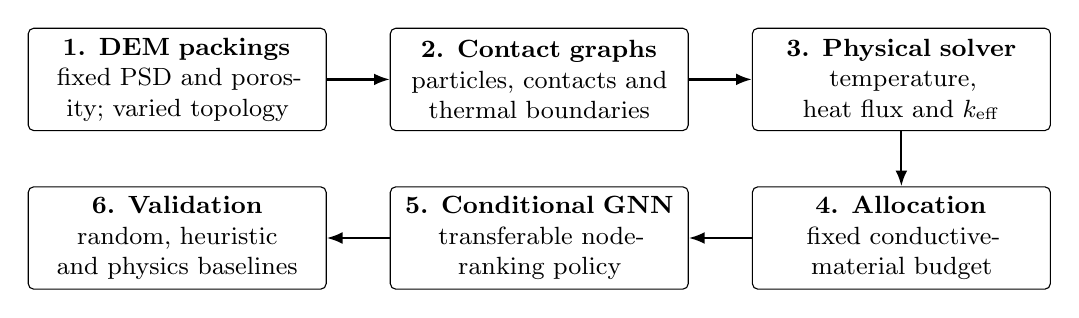
\begin{tikzpicture}[
node distance=7mm and 8mm,
box/.style={draw,rounded corners=2pt,align=center,minimum height=13mm,text width=3.55cm,font=\small},
arrow/.style={-{Latex[length=2mm]},thick}
]
\node[box] (dem) {\textbf{1. DEM packings}\\fixed PSD and porosity; varied topology};
\node[box, right=of dem] (graph) {\textbf{2. Contact graphs}\\particles, contacts and thermal boundaries};
\node[box, right=of graph] (solver) {\textbf{3. Physical solver}\\temperature, heat flux and $k_{\mathrm{eff}}$};
\node[box, below=of solver] (opt) {\textbf{4. Allocation}\\fixed conductive-material budget};
\node[box, left=of opt] (gnn) {\textbf{5. Conditional GNN}\\transferable node-ranking policy};
\node[box, left=of gnn] (test) {\textbf{6. Validation}\\random, heuristic and physics baselines};
\draw[arrow] (dem)--(graph);
\draw[arrow] (graph)--(solver);
\draw[arrow] (solver)--(opt);
\draw[arrow] (opt)--(gnn);
\draw[arrow] (gnn)--(test);
\end{tikzpicture}
\caption{Proposed workflow. DEM is run once per packing; the thermal solver can
evaluate many material allocations on the same fixed contact graph.}
\end{figure}

\section{Expected outcome and relevance}

The expected first outcome is a quantitative map of when conductive-particle
placement matters as a function of material fraction, conductivity contrast,
the competition between solid and stagnant-fluid conduction, and contact-
network realization. A useful organizing quantity is the ratio of a
characteristic contact conductance to a characteristic fluid-gap conductance.
This separates fluid-dominated, mixed-conduction and solid-network-dominated
regimes. The second outcome is an interpretable description of
effective allocations in terms of hot--cold spanning paths, bottlenecks,
parallel-path redundancy and particle/contact size. The third, conditional
outcome is a graph model that recommends an allocation on an unseen packing
without performing a long combinatorial search.

The framework is relevant to granular thermal-energy-storage media, thermally
enhanced packed beds, composite particulate materials and other systems in
which a high-conductivity additive is limited by cost, mass or processability.
Application-specific claims should be made only after selecting realistic
material pairs and including the dominant additional heat-transfer mechanisms
for that application.

\section{Principal limitations and decision points}

The intended model includes stagnant-fluid conduction but not forced convection.
This is a deliberate physical scope appropriate to static beds with negligible
fluid motion; it is not intended to represent actively ventilated or flowing
packed-bed reactors. Natural convection must be excluded through the pore-scale
Rayleigh-number check. Radiation remains negligible only at moderate
temperatures and should be added for high-temperature applications. Second, DEM
overlap is a numerical and mechanical
quantity; using it directly to calculate contact area couples the thermal result
to stiffness and confinement assumptions. Sensitivity to the conductance law is
therefore mandatory. Third, prescribing the number of high-conductivity
particles is not identical to prescribing their mass or cost when the bed is
polydisperse. The final formulation should compare number-, volume- and cost-
constrained budgets where appropriate. Fourth, ten packings are adequate for
workflow development but not necessarily for training a transferable GNN.
Finally, numerical optimization produces a theoretical material assignment;
manufacturing or mixing constraints must be added before claiming direct
experimental realizability.

\begin{thebibliography}{9}

\bibitem{Batchelor1977}
G.~K. Batchelor and R.~W. O'Brien,
``Thermal or electrical conduction through a granular material,''
\emph{Proceedings of the Royal Society of London A}, vol.~355,
pp.~313--333, 1977.

\bibitem{Vargas2001}
W.~L. Vargas and J.~J. McCarthy,
``Heat conduction in granular materials,''
\emph{AIChE Journal}, vol.~47, no.~5, pp.~1052--1059, 2001.
\href{https://doi.org/10.1002/aic.690470511}
{doi:10.1002/aic.690470511}.

\bibitem{Kiani2019}
M. Kiani-Oshtorjani and P. Jalali,
``Thermal discrete element method for transient heat conduction in granular
packing under compressive forces,''
\emph{International Journal of Heat and Mass Transfer}, vol.~145,
118753, 2019.

\bibitem{Joulin2020}
C. Joulin, A. Xiang, P. D. Lee and C. E. Krill III,
``Capturing heat transfer for complex-shaped multibody contact problems using
the discrete element method,''
\emph{Computational Particle Mechanics}, 2020.
\href{https://doi.org/10.1007/s40571-020-00321-w}
{doi:10.1007/s40571-020-00321-w}.

\bibitem{Dold2023}
D. Dold and D. Aranguren van Egmond,
``Differentiable graph-structured models for inverse design of lattice
materials,''
\emph{Cell Reports Physical Science}, vol.~4, no.~10, 101586, 2023.
\href{https://doi.org/10.1016/j.xcrp.2023.101586}
{doi:10.1016/j.xcrp.2023.101586}.

\bibitem{Battaglia2018}
P.~W. Battaglia et al.,
``Relational inductive biases, deep learning, and graph networks,''
\emph{arXiv preprint arXiv:1806.01261}, 2018.
\href{https://doi.org/10.48550/arXiv.1806.01261}
{doi:10.48550/arXiv.1806.01261}.

\bibitem{LAMMPSGranular}
LAMMPS Developers,
``\texttt{pair\_style granular} command,'' LAMMPS documentation.
\href{https://docs.lammps.org/pair_granular.html}
{docs.lammps.org/pair\_granular.html}.

\end{thebibliography}

\end{document}
